\chapter{Implementación de la aplicación}

\epigraph{\textit{''Talk is cheap. Show me the code''}}{--- Linus Torvalds}

Dentro del desarrollo de la aplicación, la parte que se puede considerar como la más importante es la parte de la implementación. Tomando en base todo el diseño, tanto a nivel conceptual, gráfico o de software, se ha implementado la aplicación, siendo esta uno de los dos objetivos del proyecto.

En este capítulo se explican los diferentes aspectos del proceso de desarrollo, tanto como se ha implementado la persistencia de datos, los escaneos que realiza la aplicación y todo tipo de consideraciones que se han tenido en cuenta durante la implementación y que merece la pena mencionar.

Este capítulo no pretende ser ni una descripción de cada elemento que forma parte del código, ni una documentación formal como puede ser la documentación de una API. Por razones de espacio y claridad, no se incluye todo el código desarrollado, tanto porque entorpecería las explicaciones de como se ha ido desarrollando y como se ha ido implementado la aplicación como porque haría este informe del proyecto excesivamente grande.

\section{Estructura del proyecto}
El código del proyecto se puede dividir en dos grandes bloques. Por una parte disponemos de los ficheros que contienen código en Kotlin y por otra parte los ficheros XML que definen, tanto layouts, elementos que se pueden dibujar o variables asociadas a las diferentes cadenas de caracteres (de ahora en adelante \textit{strings}) o a variables numéricas como colores o dimensiones.

El propio entorno de Android Studio permite diferencias ambos tipos de archivos, disponiendo del código en la carpeta \textit{java} (el nombre puede llevar a confusión, pero es el nombre por defecto en la creación de proyecto, aunque contenga únicamente código en Kotlin) y de los diferentes archivos XML en la carpeta \textit{res}. Esta última a su vez se divide en diferentes carpetas para organizar los archivos XML en función de su utilidad.

\begin{figure}[H]
	\centering
	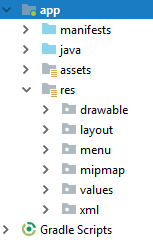
\includegraphics{basic-android-studio-structure}
	\caption{Estructura básica de archivos del proyecto}
	\label{fig:basic-android-studio-structure}
\end{figure}

Otras carpetas importantes son las carpetas de \textit{manifests} y la carpeta de \textit{assets}. En la primera es donde se guardan los diferentes \textit{Manifest} de la aplicación. Un Manifest\footnote{\url{https://developer.android.com/guide/topics/manifest/manifest-intro}} en Android es un fichero XML donde se definen una serie de variables importantes a nivel global con respecto a la aplicación. Entre otras funciones, es donde se define el nombre de la aplicación, su icono y sus diferentes componentes, que pueden ser Activities, Services, BroadcastReceivers o ContentProviders.

Por otra parte mencionar la existencia de diferentes scripts de Gradle, que es el sistema de automatización de construcción de aplicaciones más usado en Android para compilar el código y generar la aplicación ejecutable, entre otras cosas.

\subsection{Estructura de paquetes de código}

Dentro de la carpeta \textit{java}, debido a la gran cantidad de ficheros de código Kotlin, existe una estructura de paquetes que divide los ficheros de código en diferentes categorías. Cada uno de los ficheros de código existentes implementa una única clase, interfaz o tipo enumerado. Esto es así para mantener cada elemento claramente visible y al mismo nivel y a su vez evitar archivos excesivamente grandes que compliquen entender el código. La estructura de paquetes se muestra en la \autoref{fig:android-studio-package-structure}.

\begin{figure}[H]
	\centering
	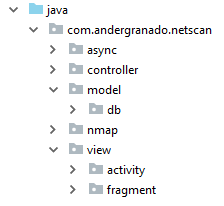
\includegraphics{android-studio-package-structure}
	\caption{Estructura de paquetes de código del proyecto}
	\label{fig:android-studio-package-structure}
\end{figure}

En los paquetes \textit{model}, \textit{controller} y \textit{view} se implementan las diferentes partes de las que está formada una aplicación que sigue el patrón MVC (Model View Controller). Es un patrón largamente usado a la hora de diseñar aplicaciones con interfaz gráfica, que consiste básicamente en dividir los datos (Model), las diferentes vistas de la aplicación (View) y la parte que actúa como puente entre los datos y las vistas (Controller) en entidades separadas. Esto permite que el codigo generado sea escalable, legible y elimine dependencias innecesarias. 

En el caso de Android, las diferentes vistas se implementan en diversas Acitivities y Fragments. El modelo es básicamente una serie de clases (algunas de ellas Data Classes de Kotlin) que definen los diferentes datos que existen, tanto para la aplicación como datos concretos que son persistentes en la aplicación (separados en el paquete \textit{db}) y los controladores están implementados usando RecyclerViews de Android, cuyo funcionamiento se explicará más adelante.

Por último, mencionar los paquetes \textit{async} y \textit{nmap}. El paquete \textit{async} contiene toda aquella funcionalidad que se ejecuta de manera paralela o asíncrona, como diferentes AsyncTasks o clases que se basan en la ejecución de Threads o hilos. El paquete \textit{nmap} contiene todo el código necesario para implementar Nmap en la aplicación, tanto para instalarlo, ejecutarlo como para interpretar los datos que genera. Todo el código que hace uso de Nmap se encuentra en este paquete, dejando el resto de la aplicación completamente aislada de las particularidades de Nmap

\section{Integración de Nmap}

Integrar soluciones de terceros en una aplicación o un sistema que está en desarrollo puede ser desde algo simple, más bien mecánico, a todo un quebradero de cabeza, en función del tipo de software o funcionalidad que queramos añadir desde fuera.

En concreto, a la hora de integrar Nmap en la aplicación hay que tener en cuenta una serie de factores. Integrar Nmap en una aplicación difiere completamente de integrar, por ejemplo, una librería con una API definida. Integrar una librería en una aplicación consiste simplemente en una serie de pasos para configurar esa librería que, una vez realizados, nos permiten mediante una interactuar mediante una API con esa librería y aprovechar toda la funcionalidad que nos provee. 

En cambio, con Nmap es radicalmente diferente. Debido a que Nmap no es una librería, sino un software complejo que nos permite analizar redes de ordenadores, no podemos integrarlo como si de una librería se tratase. Por lo tanto, debemos buscar otros métodos diferentes para integrarlo.

Nmap es una solución de código libre que lleva siendo desarrollada por la comunidad que ha generado alrededor durante más de 10 años. Cabría pensar que una posibilidad para integrar la funcionalidad de Nmap en la aplicación es obtener su código fuente (que al ser software libre es público y está disponible para su uso) e integrarlo directamente en el proyecto.

El principal problema de esta posibilidad es que Nmap es un software muy complejo. El núcleo de Nmap está desarrollado en C, pero también diversas partes están desarrolladas en lenguaje es como Lua, C++ o Python, como se puede observar en la FIGURA de su repositorio\footnote{\url{https://github.com/nmap/nmap}}. Esto impide que podamos introducir todo ese código en lenguajes no soportados por Android en el proyecto, haciendo que Nmap no se pueda integrar directamente a nivel de código.

\begin{figure}[H]
	\centering
	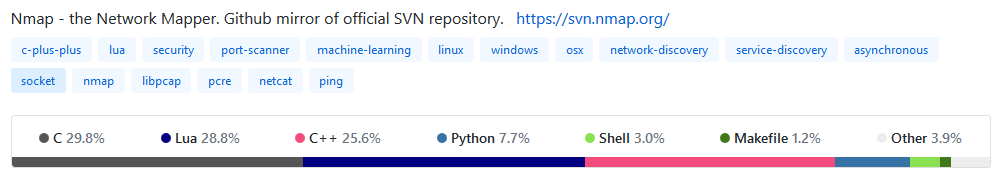
\includegraphics[width=1.0\textwidth]{nmap-repo-languages}
	\caption{Distribución de lenguajes en el repositorio de Nmap}
	\label{fig:nmap-repo-languages}
\end{figure}

Es cierto que se puede, mediante el uso del NDK de Android, introducir código tanto en C como en C++ en nuestra aplicación. Pero el funcionamiento de Nmap es tan complejo que intentar integrar solamente esa parte del código y esperar que funcione eliminando el resto de módulos sería una tarea tan titánica como inútil.

Por ello la última opción, y la única realmente viable, para integrar Nmap en nuestra aplicación es interactuar directamente con archivos binarios de Nmap. Es decir, incluir la aplicación compilada dentro del proyecto, ejecutarla mediante código y obtener e interpretar la información que devuelva.

\subsection{Instalación}

Esto a la vez genera una serie de cuestiones. Si queremos introducir un binario dentro de nuestra aplicación y controlar su ejecución en un dispositivo lo primero que tenemos que tener en cuenta es que la arquitectura para la que ha sido compilada el binario coincida con la arquitectura del dispositivo.

Nmap  es una aplicación que se puede ejecutar tanto en sistemas Windows y OS X como en sistemas basados en Linux. Aunque android es un sistema Linux, Android no se suele ejecutar en las plataformas en las que se suele ejecutar normalmente Linux, que son x86 y x64, arquitecturas Intel. La mayor parte de dispositivos Android son dispositivos con procesadores ARM BUSCAR REFERENCIA,por lo tanto no podemos  ejecutar una versión estándar de Nma para Linux.

Para solucionar esto se puede optar por dos opciones. La primera sería compilar Nmap para arquitecturas especialmente para Android en ARM. Compilar un proyecto de la envergadura de Nmap es una tarea engorrosa y difícil de realizar. La segunda sería buscar binarios ya compilados especialmente para Android. Por suerte existen binarios de Nmap para dispositivos Android.

La propia web de Nmap\footnote{\url{https://secwiki.org/w/Nmap/Android}} nos ofrece binarios de Nmap específicos para Android, la desventaja es que no se trata de binarios oficiales, aunque avalados por Nmap, sino de binarios generados por un usuario concreto\footnote{\url{https://github.com/kost/nmap-android}}. Otra desventaja de estos binarios es que no están completamente actualizados. La versión más reciente de los binarios de Nmap para Android es la 7.31 (25 de octubre de 2016), unas versiones más atrasada desde la última, la 7.70\footnote{\url{http://seclists.org/nmap-announce/2018/0}} (20 de marzo de 2018) que a día de hoy es la última versión de Nmap.

Aunque la última versión disponible de Nmap para Android no está tan actualizada como la última versión de Nmap, hay que tener en cuenta que Nmap es un software con un desarrollo avanzado y que, aunque vaya añadiendo funcionalidad, lleva durante años siendo un software robusto y estable. Por esto utilizar Nmap para Android no debería ser un gran problema.

Nmap para Android viene compilado o para una serie de arquitecturas concretas, como se puede observar en la FIGURA. Aunque tenemos un rango amplio de arquitecturas para elegir, debemos tener en cuenta que nuestro público objetivo es un público general. La mayor parte de móviles Android utilizan procesadores ARM. Aun así, y para garantizar la compatibilidad con todos los dispositivos, se han integrado binarios de Nmap para Android para arquitecturas ARM. x86 y MIPS, con sus equivalentes de 64 bits. Con esto cubriremos todos los dispositivos móviles posibles.

\begin{figure}[H]
	\centering
	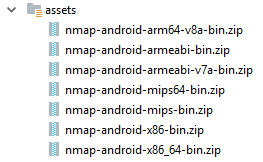
\includegraphics{project-assets}
	\caption{Los diferentes binarios para cada arquitectura usados en la aplicación}
	\label{fig:project-assets}
\end{figure}

La forma de introducir estos binarios en el dispositivo es sencilla y está completamente automatizada. por una parte se almacena cada uno de los diferentes binarios en diferentes ficheros comprimidos en formato ZIP. Cada uno de estos ficheros ZIP se encuentra metido en la carpeta \textit{assets} del proyecto, como se muestra en la \autoref{fig:project-assets}. Esta carpeta sirve para guardar todo tipo de recursos que queramos cargar en nuestra aplicación. Recursos como pueden ser ser archivos de texto, imágenes, archivos de audio, y un largo etcétera. Aunque en principio no esté diseñada para guardar binarios y programas completos, en nuestro caso servirá para guardar los ficheros de Nmap y después poder desplegarlos en el dispositivo.

Desplegarlos en el dispositivo es relativamente sencillo. Para ello solo debemos tener en cuenta la arquitectura el dispositivo en el que se está ejecutando la aplicación y descomprimir el archivo con los binarios correspondientes.

La localización donde guardemos los binarios de Nmap es fundamental, ya que según donde se guarden tendremos permiso para ejecutarlos o no. En este caso se guardan en lo que denominamos Internal Storage\footnote{\url{https://developer.android.com/training/data-storage/files}} de Android. Dentro de la estructura de archivos de Android existe una carpeta llamada \textit{data}, que a su vez tiene otra carpeta del mismo nombre. Dentro de esa última carpeta existe una carpeta por cada aplicación instalada en el sistema. Cada una contiene una aplicación y sus archivos asociados. Esta carpeta sólo es accesible para la propia aplicación, que tiene permisos de lectura, escritura y ejecución dentro de ella, lo que la convierte en el lugar idóneo para depositar los binarios.

Toda este volcado de binarios de Nmap para el dispositivo se gestiona desde una única clase en la aplicación llamada \mintinline{java}{NmapInstaller}. Esa clase, que implementa el patrón Singleton mediante el uso de la palabra clave \mintinline{java}{object} de Kotlin, contiene todo el código necesario para volcar los binarios de Nmap en el dispositivo.

\begin{code}
	\caption{Función que instala Nmap en el dispositivo}
	\label{code:install}
		
	\custominputminted{kotlin}{code/install.kt}
\end{code}

Como se puede observar en el código, dentro de la función \mintinline{java}{install()} se realiza ese volcado pudiendo tener opciones para reescribir los archivos en caso de que se quiere escribir. Estos archivos se cargan a través del Asset Manager y mediante las clases de Java para interactuar con ficheros comprimidos se extraen en los ficheros internos de la aplicación.

A su vez también se actualiza la base de datos de script NSE de Nmap, en caso de que se quiera después ejecutar alguno de esos script. 

\subsection{Ejecución}

Una vez tenemos disponibles todos los binarios de Nmap y archivos necesarios para ejecutar Nmap introducidos e instalados en el dispositivo, el siguiente paso necesario es implementar la funcionalidad que nos permita ejecutarlos.

Todo el código que permite ejecutar en el mapa se encuentra en otra clase llamada \mintinline{java}{NmapRunner}. Esta clase tiene diversos métodos que nos permiten interactuar con los binarios y en última instancia ejecutar escaneos.

Lo que tenemos que hacer para ejecutar un escaneo es ejecutar el binario de Nmap con los parámetros correspondientes. Para ejecutar en el mar basta simplemente con lanzar un proceso que llame a la ejecución del binario. La forma de ejecutar un binario es muy sencilla, y consiste en crear un proceso para una shell de Linux y en el llamar al ejecutable de Nmap. Para poder interactuar con ese proceso necesitamos configurar la entrada y la salida de ese proceso para poder enviarle información y recibirla. Eso se realizan la función \mintinline{java}{startProcess()}, que se muestra a continuación.

\begin{code}
	\caption{Función para arrancar el proceso con la shell que ejecutará Nmap}
	\label{code:startProcess}
	
	\custominputminted{kotlin}{code/startProcess.kt}
\end{code}

Después de esto debemos construir un comando de Nmap. Este comando es básicamente lo que haríamos si estuviéramos ejecutando Nmap en la terminal de nuestro ordenador. En nuestro caso solo queremos realizar una serie de escaneos concretos a nodos puntuales, por lo tanto construir este comando es tan sencillo como concatenar unos pocos strings. La función que realiza esto se muestra a continuación.

\begin{code}
	\caption{Función que crea el comando a ejecutar de Nmap}
	\label{code:commandBuilder}
	
	\custominputminted{kotlin}{code/commandBuilder.kt}
\end{code}

Una vez realizado esto queda pasar ese comando al proceso y ejecutar Nmap. A partir de aquí podríamos obtener la información del escaneo de dos maneras. La primera sería leer la salida que nos da el proceso en texto plano y extraer la información de. La segunda, mejor alternativa, consiste en ejecutar Nmap de tal manera que la información del escaneo se guarde en un fichero XML.

Las ventajas de utilizar un fichero XML para cobrar esa información son obvias. En un fichero XML dispondremos de la información estructurada que podremos leer utilizando la librería para trabajar con archivos XML que provee el SDK de Android. Por lo tanto, y como se ha podido observar, se añade el parámetro \mintinline{java}{-oX} cuándo se crea el comando a ejecutar, qué es el que indica que la salida se almacene en un fichero XML.

Una vez realizado el escaneo y habiéndose generado ese fichero XML, solo queda obtener la información de ese fichero y deshacernos de todos los recursos ya innecesarios, como el propio fichero XML una vez leído, o el propio proceso de la shell, que consume recursos no necesarios.

\begin{code}
	\caption{Función con todo el proceso de ejecución de un escaneo en Nmap}
	\label{code:runScan}
	
	\custominputminted{kotlin}{code/runScan.kt}
\end{code}

\subsection{Leer datos}

La tercera y última parte del proceso para integrar Nmap es leer los datos que han sido generados. Como se ha mencionado dichos datos se encuentran en un fichero XML. Por lo tanto, necesitaremos una clase qué obtenga la informacion de dicho fichero. A este tipo de clases se le suele denominar \textit{parser} y básicamente van leyendo las diferentes etiquetas de los ficheros XML y obteniendo su información. A continuación se muestra ciertas partes del código para hacerse la idea de cómo es leer de manera jerarquizada y estructura de un fichero XML. No se muestra toda la implementación, ya que el tamaño de la implementación de un parser de XML es directamente proporcional al tamaño de la jerarquía de los elementos que contiene.

\begin{code}
	\customtinyinputminted{kotlin}{code/nmapParser.kt}
	\caption{Extracto de la implementación de un parser de un XML de Nmap}
	
	\label{code:nmapParser}
\end{code}

Almacenar la información en XML la almacena jerarquizada en cierta manera la manera en la que Nmap guarda información estructurada en un fichero XML es como la que se muestra en el \autoref{code:regular-scan}:

\begin{code}
	\caption{Fichero XML con la información de un escaneo estándar de Nmap}
	\label{code:regular-scan}
	
	\customtinyinputminted{xml}{code/regular-scan.xml}
\end{code}

Sin entrar en detalles sobre el funcionamiento cada una etiqueta se puede observar que se genera una etiqueta \textit{host} por cada uno de los nodos encontrados en el escaneo. Un solo escaneo puede servir tanto para único host como para un rango completo de redes CIDR, por lo que habrá tantas etiquetas host como nodos se hayan detectado.

Dentro de la información generada para cada host, aunque depende del tipo de escaneo realizado, se pueden observar etiquetas que aparecerán para la gran mayoría de casos. Por ejemplo \textit{status}, que nos indica el estado del host, \textit{address}, que nos indica la dirección IP del host, \textit{hostname},que es el nombre que recibe dicho host, o la etiqueta \textit{ports}, qué contiene una lista de todos los puertos abiertos o filtrados que se han encontrado para cada nodo, con información sobre configuraciones, métodos usados para escanearlos o nombres de dichos puertos.

Por último una vez leído ese fichero a medida que se va leyendo ese fichero se va guardando la información en diferentes clases, creadas específicamente para guardar los datos obtenidos de Nmap antes de ser procesados. Dichas clases se encuentran dentro del paquete \textit{model}. En concreto, todas las clases que se usan para datos obtenidos directamente de Nmap llevan el prefijo \mintinline{java}{Nmap}, para diferenciarlas de clases del modelo relacionadas con la estructura de la información en la base de datos. En los Códigos \ref{code:nmapScan}, \ref{code:nmapHost} y \ref{code:nmapPort} se muestran unos ejemplos.

\begin{code}
	\caption{Data Classes para la información de un scan en Nmap}
	\label{code:nmapScan}
	
	\custominputminted{kotlin}{code/nmapScan.kt}
\end{code}

\begin{code}
	\caption{Data Classes para la información de un host en Nmap}
	\label{code:nmapHost}
	
	\custominputminted{kotlin}{code/nmapHost.kt}
\end{code}

\begin{code}
	\caption{Data Classes para la información de un puerto en Nmap}
	\label{code:nmapPort}
	
	\custominputminted{kotlin}{code/nmapPort.kt}
\end{code}

\section{Persistencia de datos}

A día de hoy prácticamente cualquier aplicación, independientemente de si es una aplicación móvil o una aplicación para cualquier otro sistema, requiere almacenar datos de manera persistente. Ya sea desde simples valores para guardar configuraciones o ajustes de usuario a todo un conjunto de datos que se genera, gestiona y define el funcionamiento de dicha aplicación.

En el caso de nuestra aplicación, que tiene cuyo objetivo principal analizar redes informáticas y obtener información, necesitaremos guardar la información de cada uno de esos análisis para que el usuario la tenga siempre accesible en todo momento.

La persistencia de datos una aplicación se puede implementar de diversas maneras, y la elección de una manera u otra obedece a varios factores. Hay que tener en cuenta, entre otras cosas, el volumen de datos que se vaya a generar, la frecuencia con la que se van a modificar esos datos o si esos datos van a ser transferidos en algún momento.

A grosso modo se pueden dividir las formas de implementar persistencia de datos en dos principales tipos: el uso de ficheros o el uso de bases de datos.

El uso de ficheros es el modo más simple de almacenar datos. Consiste en guardar los datos escribiendo en ficheros y en obtener datos leyendo de ellos. Esos ficheros pueden contener los datos en sí mismos o junto a algún tipo de estructura, siendo esta la más sencilla de mantener. Como ejemplos de datos estructurados tenemos una serie de formatos como XML, CSV o JSON.

Por otra parte, tenemos el uso de bases de datos. A medida que los datos crecen en complejidad y en número, se vuelve cada vez más complicado el acceso lectura y escritura dichos datos. El uso de bases de datos permite almacenar una gran cantidad de datos relacionados entre ellos, de los cuales podemos obtener información concreta y modificar la información más concreta mediante lenguajes como SQL.

A la hora de elegir entre una de las dos para nuestra aplicación debemos tener en cuenta que el uso de bases de datos permite mayor escalabilidad y nos permite gestionar mejor los datos que son generados. Aun añadiendo otra capa más, como es sistema de gestión de bases de datos, que a priori resulta más costoso computacionalmente respecto al uso de ficheros, a la larga va a ser la mejor opción para guardar los datos de nuestra aplicación.

Una vez elegido que vamos a implementar la persistencia de datos usando bases de datos el siguiente paso a realizar es  elegir qué sistema de gestión de bases de datos vamos a utilizar. En este caso la elección resulta bien sencilla. El propio SDK de Android implementa funcionalidad para poder trabajar con bases de datos SQLite. SQLite es un sistema de gestión de bases de datos relacional basado en SQL qué es conocido por ser ligero y eficiente.

\subsection{Diseño de la base de datos}

El diseño de nuestra base de datos resultado sumamente simple. Únicamente queremos guardar la información de una serie de escaneos. Sabemos que un escaneo al final está compuesto de la información de una serie de nodos y, a su vez, de cierta información secundaria, como la fecha que se la que se ha hecho o el nombre de la red. Cada nodo tiene su propia información, desde el fabricante del dispositivo a la dirección IP o la lista de puertos que tiene abiertos, entre otros. El modelo que se plantea para esta base datos es sumamente sencillo y se muestra en la \autoref{fig:db-tables}.

\begin{figure}[ht]
	\centering
	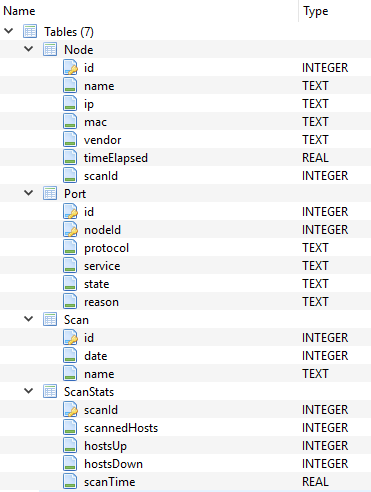
\includegraphics{db-tables}
	\caption{Arquitectura de Room e interrelación entre sus diferentes componentes}
	\label{fig:db-tables}
\end{figure}

Cómo podemos observar solo contamos únicamente con cuatro tablas (se han omitido las tablas generadas automáticamente por Android). Una para cada escaneo, otra para las diferentes estadísticas sobre cada escaneo, otra para que la información de cada nodo y una última para la información de de un puerto de un nodo concreto. Este caso se ha optado por almacenar esta información, pero resultaría fácilmente escalable simplemente añadiendo más campos en nuestra base de datos.

\subsection{Implementación de la base de datos}

Tras tener la base de datos diseñada debemos implementar la nuestra aplicación. Implementar una base de datos en Android se puede hacer de dos maneras.La primera, la manera tradicional, es utilizar la API estándar de Android para interactuar con bases de datos SQLite. Esta manera implica que debemos introducir nuestras sentencias SQL y ejecutarlas nosotros mediante las diferentes funciones y métodos que nos ofrece la API.

Una alternativa a esta API estándar sería el uso de la librería \textit{Room}\footnote{\url{https://developer.android.com/topic/libraries/architecture/room}}. Esta librería es una de las librerías que forman parte de lo que sedenomina Android Architecture Components. los Architecture Components son diferentes librerías pensadas para solucionar problemas que surgen a la hora de desarrollar aplicaciones en Android y simplificar en gran medida el desarrollo de ciertos tipos de funcionalidad.

Room está pensado para abstraernos de toda la lógica de SQL y permitirnos interactuar con la base de datos de una manera más limpia y natural. A abstraer toda esa capa de composición de sentencias SQL para realizar nuestras consultas y modificaciones de la base de datos, el código a mantener resulta muchísimo más sencillo y elegante.

Para lograr esto se basa en una arquitectura compuesta de tres bloques o componentes principales. Dicha arquitectura se puede observar en la FIGURA.

\begin{figure}[H]
	\centering
	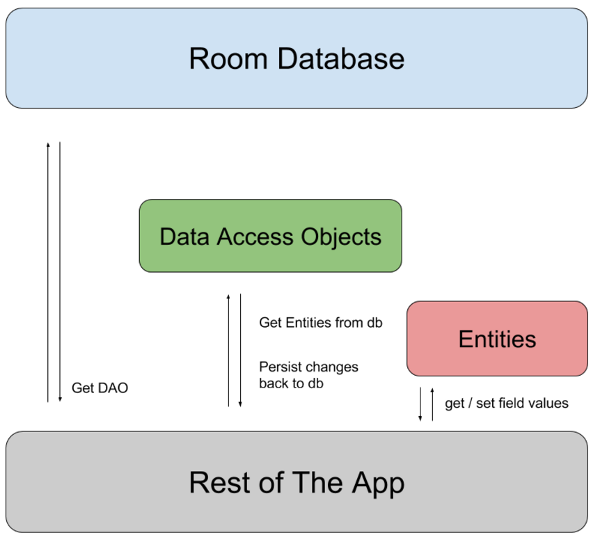
\includegraphics[width=\textwidth]{room-architecture}
	\caption{Arquitectura de Room e interrelación entre sus diferentes componentes}
	\label{fig:room-architecture}
\end{figure}

El primero es el componente \textit{Database}. Este componente es el que nos permite realizar tareas con la base de datos a nivel global. Desde definir las diferentes tablas que pueda haber a obtener la instancia de la base de datos para poder trabajar con ella.

\begin{code}
	\caption{Implementación de la clase AppDatabase}
	\label{code:roomDatabase}
	
	\custominputminted{kotlin}{code/roomDatabase.kt}
\end{code}

En el código \ref{code:roomDatabase} se muestra la  implementación de ese componente en nuestra aplicación. Aún no habiendo visto nunca cómo funciona Room se pueden incluir ciertas cosas examinando el código. La primera es que se define mediante anotaciones ciertas clases. Esas clases son las que definen cada una de las tablas que vamos a tener en nuestra base de datos. En Room, las tablas son conocidas como \textit{Entities}, que es otro de los tres componentes de Room. También se puede observar que se añaden una serie de funciones que contienen la nomenclatura \textit{DAO}. Esas funciones son las que nos van a permitir obtener los diferentes DAOs que puedan existir en Room, siendo este tipo de componente el tercero y último.

Como se ha mencionado, las Entities corresponden a cada una de las tablas que existe en la base de datos. Para reflejar esto en una clase de tipo Entity, de la misma manera que se hacía para el componente Database, se utilizan anotaciones.

\begin{code}
	\caption{Implementación de diferentes clases Entity}
	\label{code:roomEntities}
	
	\custominputminted{kotlin}{code/roomEntities.kt}
\end{code}

Cómo se puede observar en el ejemplo que se ha puesto en el CÓDIGO, se utilizan anotaciones para definir una entidad o para definir aspectos como la clave primaria de una tabla de la base de datos. Cada uno de los atributos de esa clase equivaldría a un campo de la tabla. Los tipos de datos de la tabla equivalen a los tipos de datos que se han utilizado en los atributos de la clase. Para tipos de atributos complejos Room implementa un componente llamado \textit{Converters} que nos permite implementar funciones que convierten tipos de datos complejos, como imágenes, datos personalizados o clases complejas, en tipos de datos almacenables en una base de datos, de tal manera que se ejecuten automáticamente a la hora de interactuar con la base de datos.

Por último, el tercer componente que se ha mencionado son los \textit{DAO} (Data Access Object). Estos componentes son interfaces que definen una serie de funciones. Esas funciones son la que se utilizarán para hacer consultas o modificaciones en la base de datos. El uso de sentencias SQL como \textit{SELECT}, \textit{INSERT}, \textit{UPDATE} o \textit{DELETE} queda encapsulado mediante el uso de estas funciones, que tanto reciben como devuelven, dependiendo el caso, tipos de datos manipulables a nivel de código. Cada interfaz DAO permite interactuar con una o mas tablas, siendo lo mas recomendable implementar una para cada tabla definida.

\begin{code}
	\caption{Ejemplo de una interfaz DAO para interactuar con la base de datos}
	\label{code:roomDao}
	
	\custominputminted{kotlin}{code/roomDao.kt}
\end{code}

Como se puede apreciar en el código \ref{code:roomDao}, mediante anotaciones es donde se especifican las sentencias SQL a las que equivale la ejecución de esas funciones.

Por lo tanto para ejecutar algún tipo de operación en la base datos simplemente hay que combinar estos tres elementos, para disponer de herramientas para definir el modelo de la base de datos e interactuar con la instancia de la base de datos. Por poner unos ejemplos, en los códigos \ref{code:roomSelect} y \ref{code:roomInsert} se muestran partes concretas de la aplicación en las que se realiza una consulta y una inserción en la base de datos, respectivamente.


\begin{code}
	\caption{Ejemplo de obtención de información de la base de datos Room}
	\label{code:roomSelect}
	
	\custominputminted{kotlin}{code/roomSelect.kt}
\end{code}

\begin{code}
	\caption{Ejemplo de inserción de información en la base de datos Room}
	\label{code:roomInsert}
	
	\custominputminted{kotlin}{code/roomInsert.kt}
\end{code}

Se ha podido ir percibiendo, en ningún momento se ha implementado código que realmente ejecute sentencias SQL. Aquí reside la magia de Room. Room abstrae completamente la programación de ese tipo de código siendo la propia librería quién se encarga de generar ese código a la hora de compilar la aplicación.

Las ventajas de utilizar Room con respecto a la API estándar de SQLite son obvias. Tanto es así que la propia documentación ''recomienda encarecidamente usar Room en vez de SQLite''\cite{room-training}. En primer lugar, abstraemos completamente la generación de código donde concatenamos, generamos y ejecutamos sentencias SQL. Por otra parte, el código que gestiona la base de datos resulta mucho más claro y conciso limitándose a consistir en un par de llamadas a funciones. Por último, la creación de las tablas de la base de datos en sí misma se hace también de manera automática. Incluso tenemos herramientas para poder generar diferentes versiones de la propia base datos a medida que la aplicación vaya escalando, guardándose historiales de versiones de la base de datos para en caso de revertir cambios volver a la estructura de una de las bases de datos anteriores.

\section{Obtención de información de medios externos}

Gracias al uso de Nmap podemos obtener información de los diferentes nodos de las redes a escanear. Aún así, a causa de varios factores, necesitamos adquirir partes concretas de información desde medios externos.

\subsection{Obtención del fabricante de un nodo de la red}

Uno de los puntos fuertes de nuestra aplicación es el que al escanear los nodos de la red, podamos identificar el fabricante del dispositivo escaneado. El problema es que Nmap únicamente es capaz de hacer esto si es capaz de conocer la dirección de hardware (también conocida como dirección MAC o dirección física) del dispositivo que está escaneando. Debido a que, por el propio funcionamiento de Nmap, solo puedo obtener la dirección de hardware si se tiene privilegios de superusuario, esa información no podemos obtenerla directamente mediante el uso Nmap.

Para ello, y como alternativa, se ha programado la obtención de la dirección de hardware de manera manual. La obtención de esta dirección de hardware se realiza analizando la información de las tablas ARP. ARP es un protocolo de comunicaciones responsable de encontrar la dirección de hardware que corresponde a una determinada dirección IP.  las tablas ARP son las que contienen la información que relacionan esas direcciones de hardware con las direcciones IP. Mediante un sencillo código, implementado en una función, podemos leer este fichero, que no deja de ser un fichero de texto plano, y obtener dicha MAC de manera sencilla, y juntarla al resto de la información del nodo para finalmente insertar dicha información en nuestra base de datos. Se peude observar la implementación en el Código \ref{code:getMac}.

\begin{code}
	\caption{Código que obtiene la dirección física en base a una dirección IP}
	\label{code:getMac}
	
	\custominputminted{kotlin}{code/getMac.kt}
\end{code}

Tras obtener la dirección MAC, necesitamos, en base a ella, obtener el fabricante del dispositivo. Esto es posible debido a que el reparto de direcciones MAC está regulado y a la hora de establecer una interfaz de red en un dispositivo, que va a tener una dirección de hardware única, el fabricante necesita previamente un espacio de direcciones MAC para sus dispositivos.

Cabe recordar que una dirección MAC está formada por 48 bits y se suele representar con cada uno de sus 6 bytes en hexadecimal, separados entre ellos por dos puntos. Dentro de esta dirección de hardware, los tres primeros bytes, es decir la primera mitad de la dirección de hardware, corresponde a un único fabricante, que tiene permiso para distribuir dispositivos con direcciones de hardware que comiencen por esos 3 bytes. Al estar reguladas estas direcciones de hardware, solo debemos buscar en algún medio externo esa información. Dicha información la provee directamente ICANN (Internet Corporation for Assigned Names and Numbers), que es una entidad que se encarga de repartir direcciones IP y MAC, entre otras cosas.

En nuestro caso concreto utilizamos la información de un fichero de texto\footnote{\url{https://code.wireshark.org/review/gitweb?p=wireshark.git;a=blob_plain;f=manuf}} contenido en las bases de datos de Wireshark Foundation, conocida empresa por el desarrollo del programa Wireshark (qué se utiliza para sniffing de paquetes de una red). Este archivo lo bajamos directamente de Internet y en base a él obtenemos información del fabricante. El archivo tiene el formato que se muestra en el fichero \ref{code:ouis-txt}. 

\begin{code}
	\caption{Extracto del fichero que relaciona direcciones MAC on fabricantes}
	\label{code:ouis-txt}
	
	\custominputminted{kotlin}{code/ouis.txt}
\end{code}

Para gestionar la descarga la lectura y cotejar la dirección MAC con esa información obtenida mediante el archivo se han implementado varias partes. Lo primero es una interfaz genérica conocida como \mintinline{kotlin}{DownloadableResource}. Esta clase abstracta simplemente define una serie de variables y métodos para implementar clases que sirvan para descargar un recurso de Internet.

\begin{code}
	\caption{Clase abstracta para un recurso descargable}
	\label{code:downloadable}
	
	\custominputminted{kotlin}{code/downloadable.kt}
\end{code}

Cómo se puede observar en el Código \ref{code:downloadable}, se definen funciones para descargar un archivo mediante el uso de un \textit{Thread} o hilo. El descargar el archivo mediante el uso de un hilo, es decir de manera paralela a la ejecución de la aplicación, es necesario ya que por motivos de usabilidad, Android por defecto no permite realizar operaciones de red en el principal de la aplicación (lanzando en caso de hacerlo una excepción de tipo \mintinline{kotlin}{NetworkOnMainThreadException}). El Thread principal está exclusivamente reservado a la ejecución de operaciones relacionadas con la interfaz. De esta manera, no se bloqueará la ejecución de la aplicación simplemente por estar descargando un archivo. 
Por otro lado, el crear esta clase abstracta o interfaz permite en un futuro, si es necesario, implementar más recursos de este tipo para obtener información de diferentes fuentes.

En este caso concreto heredado de esta clase abstracta, creando una nueva clase (que implementa el patrón Singleton) llamada \mintinline{kotlin}{OUIs}. Esta clase contiene todos los métodos para gestionar la descarga de fichero de texto, además funciones para obtener, en base a una dirección MAC, el fabricante del dispositivo analizado. Esto se hace de manera muy sencilla, recorriendo el archivo, leyendo los valores e identificando las direcciones MAC hasta encontrar el resultado, como se puede ver en el Código \ref{code:getVendor}.

\begin{code}
	\caption{Obtención el fabricante en base a la dirección MAC}
	\label{code:getVendor}
	
	\custominputminted{kotlin}{code/getVendor.kt}
\end{code}

También de manera análoga a la obtención del fabricante de un dispositivo se ha obtenido información sobre diferentes puertos.

La información que da sobre un puerto Nmap resulta de utilidad, pero no permite entender para qué sirve ese puerto. Se puede llegar a conocer el funcionamiento de puertos comunes, como el puerto 80, utilizado para HTTP, o el puerto 22, utilizado para SSH. Pero en caso de tratarse de otros puertos menos usuales algo de información textual resulta de gran ayuda. Mediante Nmap sólo podemos obtener el nombre que tiene ese puerto (a parte de información sobre su estado, etc.). Para obtener información textual podemos usar otra fuente de información, que casualmente también se ha obtenido de ICANN. 

Obtener información de este archivo es ligeramente más complicado, ya que no se trata simplemente de un fichero de texto sino de un fichero XML, con una estructura información más compleja. De todas maneras la descarga del archivo y la gestión de activos se realiza de la misma manera, ya que hemos implementado una clase abstracta que define cómo tenemos que hacerlo. Por otro lado, para la lectura del archivo XML se utiliza otro parser de XML, mucho más sencillo que el que se utiliza para leer la información de Nmap, pero que está implementado de la misma manera.

Todo esto se ha implementado en otra clase (también Singleton) para poder, mediante métodos concretos (como se hacía a la hora de obtener el fabricante), indicarle un puerto y obtener más información textual sobre dicho puerto.

% TODO: Añadir el codigo
%\begin{code}
%	\caption{Obtención información del objetivo de un puerto concreto}
%	\label{code:getServiceName}
%	
%	\custominputminted{kotlin}{code/getServiceName.kt}
%\end{code}
\begin{code}
	\caption{Obtención información del objetivo de un puerto concreto}
	\custominputminted{kotlin}{code/placeholder.kt}
\end{code}

En este caso se han implementado estos dos sistemas para obtener información desde medios externos, pero debido a la manera en la que están implementados, mediante esa interfaz abstracta, implementar más métodos de obtención de datos de terceras partes resulta bastante sencillo.

Por último mencionar que estos elementos contienen relativamente una gran cantidad información, pero al ser información en formato texto plano o XML, descargarlos no resulta costoso. Además, por conveniencia, se ha optado por lanzar las descargas de estos archivos en el momento en el que arranca la aplicación. De esta manera los archivos estarán descargados cuando queramos utilizarlos, de una manera completamente transparente al usuario, sin que tenga que hacer absolutamente nada.

Se ha optado por utilizar este modelo (descargar en cada inicio de la aplicación toda la información de medios externos), y no guardarla de manera persistente en nuestra aplicación. Esto es debido principalmente a que descargarla no es una tarea demasiado costosa y podemos tener siempre la información actualizada. Esto requiere que siempre que lancemos la aplicación se tenga conexión a Internet, pero como vamos a requerir de dicha conexión para aprovechar cualquiera de las funcionalidades, esa conexión, de una manera u otra, siempre va a ser necesaria.

\section{Hilos, Tareas y paralelización}

Un aspecto también fundamental para entender el comportamiento de la aplicación es todo lo relacionado con la ejecución de hilos, tareas o procesos. Si bien esta aplicación en no se trata de una aplicación que esté basada en multithreading o programación paralela, se hace uso de diferentes técnicas relacionadas en ciertos puntos de la implementación. En los próximos parrafos se indagará en dichos aspectos.

Por una lado (y esto es un aspecto que ya se ha mencionado previamente), la ejecución de Nmap es completamente independiente a la ejecución de la aplicación. Android, como cualquier sistema operativo basado en Linux,tiene como elementos fundamentales de ejecución los procesos. Esto quiere decir que, en el sistema, tendremos todo tipo de procesos corriendo. Esos procesos pueden corresponder a aplicaciones o ser procesos del propio sistema operativo. En este caso la ejecución del binario de Nmap se lanza en un proceso independiente, uniéndose al resto de procesos que se están ejecutando en ese momento en el dispositivo.

El proceso de Nmap no consiste únicamente en la ejecución del binario. El proceso en sí que se lanza consiste en la ejecución de una \textit{shell}, dentro de la cual se lanzarán los comandos que permitan ejecutar Nmap. Por lo tanto, no es que tengamos un proceso de ejecución, sino que tenemos una shell asociada que tendrá configuradas tanto la entradas como la salida para que se comuniquen con nuestra aplicación. Comunicar la entrada y la salida de un proceso es bastante sencillo, y se realiza de manera similar a como se haría con un archivo, como se muestra en el Código \ref{code:startProcess2}.

\begin{code}
	\caption{Creación del proceso, la entrada y salida para Nmap}
	\label{code:startProcess2}
	
	\custominputminted{kotlin}{code/startProcess.kt}
\end{code}

En este caso concreto lo más importante es la entrada, porque es la forma en la que lanzaremos los comandos de Nmap, y por ende, ejecutar la aplicación. La salida, en este caso, no resulta importante ya que lo que hacemos al ejecutar Nmap es indicar que los resultados se guarden en un fichero XML, por lo tanto aunque tengamos abierta la salida de ese proceso y redirigida a nuestra aplicación, en principio no se hará uso de ella, únicamente para tareas puntuales de depuración.

Otro de los aspectos, que también se ha mencionado ya en otras secciones, es el relacionado con los hilos o Threads de ejecución. Teniendo en cuenta que no se puede ejecutar operaciones de red en el hilo principal de ejecución de la aplicación (al menos por defecto), se han implementado ciertas partes mediante el uso de Threads. Principalmente lo que se ha implementado mediante Threads son las descargas de los diferentes archivos que se utilizan para obtener información de medios externos. Se ha programado mediante Threads de Android (que viene a ser Threads de Java) y no mediante otros mecanismos de ejecución asíncrona de código debido a la simplicidad de la implementación de un Thread y también porque las tareas a realizar no tienen complejidad a nivel de programación. Consisten en descargar y leer archivos de Internet, lo que, como se puede comprobar en el Código \ref{code:downloadThread}, se puede hacer con unas pocas líneas de código.

\begin{code}
	\caption{Ejecución de la descarga y lectura de un archivo en un Thread}
	\label{code:downloadThread}
	
	\custominputminted{kotlin}{code/downloadThread.kt}
\end{code}

El tercer y último bloque dentro de toda la parte de ejecución asíncrona y paralelización de código es el usado a la hora de actualizar la interfaz gráfica. Android, al igual que muchísimos sistemas, utiliza el patrón de diseño MVC. Esto tiene una serie de ventajas, permitiendo separar la presentación o vista de la aplicación de la lógica o modelo. Con ello se logra separar la vista del resto, permitiendo poder modificarla en todo momento de manera independiente.

La vista se comunica con el modelo a la hora de obtener datos mediante el uso de controladores. La forma más sencilla de cargar nuestra vista con los datos que contiene el modelo es obtener los datos del modelo interactuando con el controlador cuándo se realiza la creación de la vista.

Esto en ciertas partes de la aplicación es viable, como por ejemplo en la parte en la que mostramos la lista de escaneos realizados o la parte en la que visualizamos los diferentes nodos de un escaneo concreto. En ambos casos se da la situación en la que lo que hacemos es, a la hora de cargar el Activity o el Fragment, Usar el controlador para comunicarnos con el modelo y obtener los datos para mostrarlos desde un principio.

Pero hay casos en los que esto no es posible. El caso más importante a tener en cuenta es  cuando se está realizando el escaneo de una red. Al realizar el escaneo de una red vamos a tener a Nmap ejecutándose y iremos obteniendo la información que vaya sacando. Para implementar esto se pueden hacer varias aproximaciones.

La primera sería lanzar la ejecución de Nmap, realizar el escaneo completo de la red (esperando mientras se realiza) y obtener la información que ha generado. El principal inconveniente de esta aproximación consiste en que no tendríamos ningún tipo de salida hasta que no terminase el escaneo completo. Esto quiere decir que no se visualizará ningún cambio en la Activity hasta finalizar. Claramente es negativo, ya que dejaríamos al usuario sin información durante un tiempo de espera muy grande. 

Otra aproximación, mejor que la primera, sería ir obteniendo partes de la información e ir mostrándola en pantalla. Para realizar esto necesitamos lanzar una tarea que se ejecute de manera asíncrona y vaya realizando los escaneos por partes. Perdemos esa sencillez que nos da el hecho de escanear toda la red mediante una única ejecución de Nmap, pero ganamos la flexibilidad de poder ir obteniendo la información poco a poco.

Para ello se hará uso de un \textit{AsyncTask}\footnote{\url{https://developer.android.com/reference/android/os/AsyncTask}} de Android. Un AsyncTask es un método para ejecutar una tarea de manera asíncrona en Android. Para implementar una tarea asíncrona, debemos heredar de esta clase e implementar las diferentes funciones que pide implementar. Un ejemplo vacío de la clase se muestra en el Código \ref{code:asyncTask}.

\begin{code}
	\caption{Ejemplo de la estructura de una AsyncTask}
	\label{code:asyncTask}
	
	\custominputminted{kotlin}{code/asyncTask.kt}
\end{code}

Las funciones que requiere implementar son cuatro, y se enumeran a continuación:

\begin{enumerate}
	\item \mintinline{kotlin}{onPreExecute()}: Se invoca antes de ejecutarse. Normalmente se usa para inicializar valores o preparar lo necesario para la ejecución.
	\item \mintinline{kotlin}{doInBackground(Params…)}: Se invoca ya en un Thread aparte y es donde se realiza el contenido de la tarea. Dentro de ella, se llama a la función \mintinline{kotlin}{publishProgress(Progress...)} en caso de que se quiera indicar algún tipo de progreso.
	\item \mintinline{kotlin}{onProgressUpdate(Progress…)}: Se ejecuta cuando se ha recibido algón tipo de progreso. Normalmente se usa para actualizar la interfaz gráfica e indicar al usuario que se ha realizado progresos.
	\item \mintinline{kotlin}{onPostExecute(Result)}: Se ejecuta una vez la tarea ha terminado, y permite interactuar con el resultado
\end{enumerate}

La implementación de una AsyncTask permite que podamos usar el tipo de datos que queramos tanto para \mintinline{kotlin}{Params}, \mintinline{kotlin}{Progress} o \mintinline{kotlin}{Result}, o ninguno rn caso de no necesitar algunos de ellos.

Para el caso concreto de la aplicación, se han implementado varias tareas asíncronas. La primera de ellas, \mintinline{kotlin}{NetworkScan} (mostrada en parte en el Código \ref{code:networkScan}, sirve como base para definir diferentes tipos de escaneos, y en ella se implementa funcionalidad común para cualquier tipo de escaneo. Esta clase, como se muestra en CÓDIGO es abstracta y no puede ser instanciada.

\begin{code}
	\caption{Implementación de metodos de una AsyncTask en la clase NetworkScan}
	\label{code:networkScan}
	
	\custominputminted{kotlin}{code/networkScan.kt}
\end{code}

Basándonos en \mintinline{kotlin}{NetworkScan}, la implementación más sencilla de un escaneo de una red está programada en la clase \mintinline{kotlin}{SequientialNetworkScan}. En esa clase, como se puede observar en el Código \ref{code:sequentialNetworkScan}, ya se implementan las llamadas a Nmap y el guardado en la base de datos. El nombre de la clase viene dado porque realiza el escaneo de manera secuencial, es decir, uno por uno.

\begin{code}
	\caption{Implementación de parte de la tarea asíncrona SequentialNetworkScan}
	\label{code:sequentialNetworkScan}
	
	\customtinyinputminted{kotlin}{code/sequentialNetworkScan.kt}
\end{code}

También se puede observar que esta clase, al igual que la clase base, también es abstracta, ya que consiste en una implementación abstracta, únicamente con la lógica del escaneo de Nmap. Para poder realizar un escaneo, debemos implementar una subclase de ésta dentro de la vista (ya se Activity o Fragment) en la que queramos mostrar los datos. De esta manera, las particularidades de la vista y de cómo se cargan los datos en ella quedan relegados a código dentro de la vista, manteniendo el uso del patrón MVC. La implementación interna en una Activity quedaría como se muestra en el \ref{code:innerNetworkScan}, y, como se puede apreciar, solo contiene código relacionado con la interfaz de usuario.

\begin{code}
	\caption{Implementación de un NetworkScan dentro de un Activity}
	\label{code:innerNetworkScan}
	
	\custominputminted{kotlin}{code/innerNetworkScan.kt}
\end{code}

Para lanzar una tarea asíncrona simplemente debemos, una vez construido el objeto, llamar al un método llamado \mintinline{kotlin}{Execute()}. Ejecución que solo se podrá realizar una vez para cada instancia, debido a las características internas de un AsyncTask, para evitar que una tarea ya realizada se vuelva a realizar.

En conclusión, se ha desarrollado un modelo que permite, por una parte, separar la lógica de la interfaz gráfica y, por otra parte, disponer de una jerarquía extensible que permite realizar diferentes tipos de escaneos. Una jerarquía de clases que se pueden extender para realizar escaneos mediante otros métodos, como pueden ser ejecuciones en paralelo u otro tipo de implementaciones.


\section{Interfaz gráfica}


